


\subsection{Inverted F-antenna}\label{sec:ifa_sim}




The inverted F-antenna (IFA) is modeled in Ansys HFSS as shown in \autoref{fig:ifa}. Its material is copper. It is positioned at the center of the TEM cell, mounted at the top surface. The 5\,mm long wire points towards waveport 2. The excitation is a modal wave port. With a maximum dimension of 5\,mm, the antenna is electrically small for a frequency of up to 6\,GHz, at which it will be a tenth of the wavelength. In this simulation, the antenna is investigated for the frequency of 100\,MHz to 1\,GHz. The TEM cell has a width of 40\,mm and a height of 24\,mm. The goal is to find equivalent dipole moments. 


\begin{figure}[h]
    \centering
    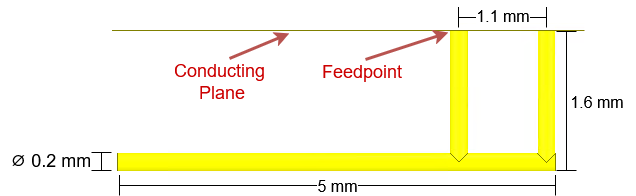
\includegraphics[width=0.75\linewidth]{Documentation//content//30_simulations//img/inverted_f_antenna.png}
    \caption{Inverted F-antenna used in the simulation}
    \label{fig:ifa}
\end{figure}

The coupling between the antenna and the two ports of the TEM cell are described by S-parameters, specifically the forward transmission coefficients $S_{\mathrm{A1}}$ and $S_{\mathrm{A2}}$. \autoref{fig:antenna_waveport1_sparams} shows the magnitude of this coefficient, which is the same for the antenna to both ports. The phase shifts of $S_{\mathrm{A1}}$ and $S_{\mathrm{A2}}$ differ, which is shown in \autoref{fig:phase_shift_waveports_ifa}. This phase shift delivers important information about the equivalent dipole moments.
 

\begin{figure}[h]
    \centering
    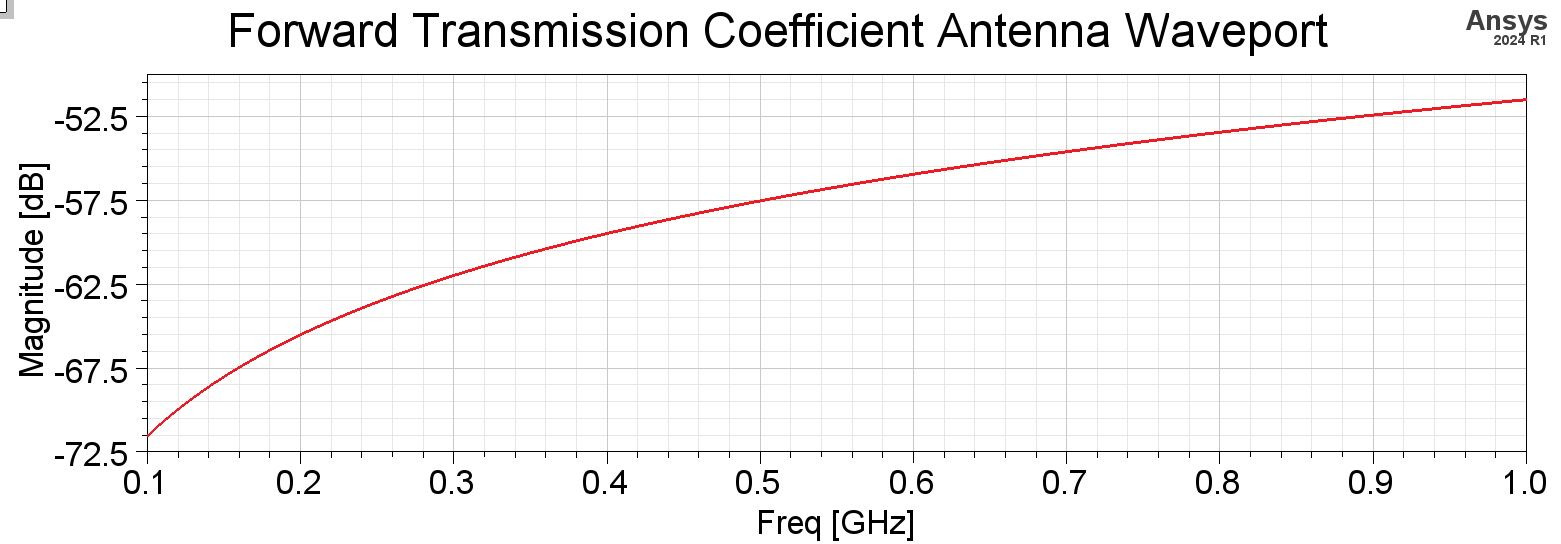
\includegraphics[width=1\linewidth]{Documentation//content//30_simulations//img/antenna_waveport1_sparams.png}
    \caption{S-Parameter describing coupling of antenna to waveport 1}
    \label{fig:antenna_waveport1_sparams}
\end{figure}

\begin{figure}[h]
    \centering
    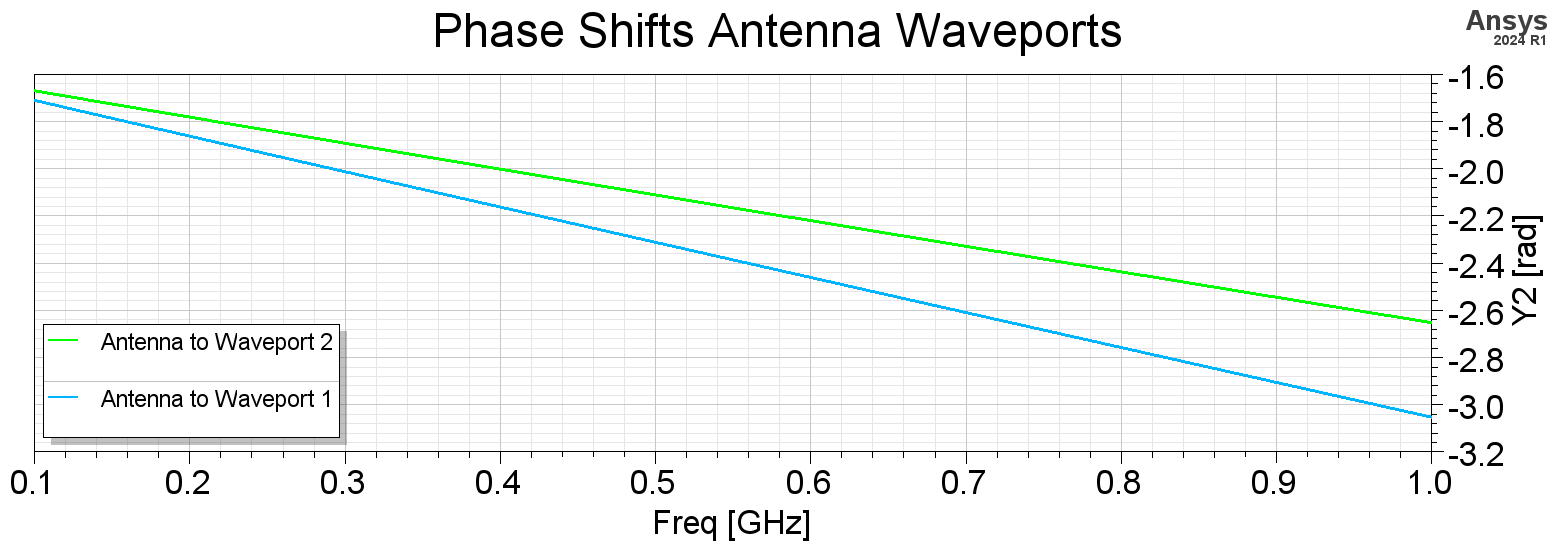
\includegraphics[width=1\linewidth]{Documentation//content//30_simulations//img/Phase Shift Waveports.png}
    \caption{Phase of S-parameters from antenna to waveport 1 and 2}
    \label{fig:phase_shift_waveports_ifa}
\end{figure}


\begin{equation}
    P_{\mathrm{Antenna}}=\frac{P_{\mathrm{Out1}}}{10^{|S_{\mathrm{A1}}|/10}}=\frac{P_{\mathrm{Out2}}}{10^{|S_{\mathrm{A2}}|/10}}
    \label{eqn:power_antenna}
\end{equation}


\autoref{eqn:power_antenna} describes the relation between the input power at the antenna and the measured output power of the TEM cell. It is defined by the magnitude of the forward transmission coefficients.

\begin{equation}
    \iint_A \mathbf{e_0} \times \mathbf{h_0} \cdot\mathrm{d}\mathbf{A} = 1
    \label{eqn:normalization of fields}
\end{equation}

\autoref{eqn:normalization of fields} shows that the electric field $\mathbf{e_0}$ and magnetic field $\mathbf{h_0}$ are normalized to $1\,\sqrt{\mathrm{W}}$. The surface area $A$, over which the fields are integrated, is that of the output ports of the TEM cell. The field can be linearly scaled by the coefficients $a$ and $b$, which has been described in \autoref{eqn:modal_superposition1} and \autoref{eqn:modal_superposition2}. Only one pair of such coefficients is needed, since only the TEM mode is considered. The coefficients $a$ and $b$ have the unit $\sqrt{\mathrm{W}}$. The fields $\mathbf{e_0}$ and $\mathbf{h_0}$ are not known over the whole area. However, the electric field $\mathbf{e_0}$ has only to be known at one specific point in order to determine the equivalent dipole moments, as will be shown here.

\begin{subequations}
\begin{equation}
    P_{\mathrm{out1}}=\iint_A \langle \mathbf{S} \rangle \cdot \mathrm{d}\mathbf{A}= \iint_A \frac{1}{2} \, \Re \{ \left(a\cdot \mathbf{e_0}\right) \times \left(a\cdot \mathbf{h_0}^*\right) \}\cdot \mathrm{d}\mathbf{A} = \frac{|a|^2}{2}
    \label{eqn:power_of_poynting1}
\end{equation}
\begin{equation}
    P_{\mathrm{out2}}=\iint_A \langle \mathbf{S} \rangle \cdot \mathrm{d}\mathbf{A}= \iint_A \frac{1}{2} \, \Re \{ \left(b\cdot \mathbf{e_0}\right) \times \left(b\cdot \mathbf{h_0}\right)^* \}\cdot \mathrm{d}\mathbf{A} = \frac{|b|^2}{2}
    \label{eqn:power_of_poynting2}
\end{equation}
\end{subequations}
\todo{linear relation Power to b, a}

The output power of each port is then derived through \autoref{eqn:power_of_poynting1} and \autoref{eqn:power_of_poynting2}. So if $a=b=1$, then the electric field $\mathbf{e_0}$ may be measured, when the output power at one port is $\frac{1}{2}\,\mathrm{W}$. Because it is assumed that the TEM cell contains only waves in the TEM mode, the normalization of the electric and magnetic fields can be used to simplify the calculations.

\begin{equation}
    \mathbf{e_0}\times\mathbf{h_0}=\Re\{\mathbf{e_0}\times\mathbf{h_0}^*\} \quad\text{for TEM mode}
    \label{eqn:equivalent_tem}
\end{equation}

\todo{Problem with large TEM cell: Formula does not work for large frequencies. The field distributes around the port. Describe this. Error grows with frequency}

By using \autoref{eqn:mag_dipole_moment_tem} and \autoref{eqn:dipole_tem_waves}, the equivalent dipole moments are derived. Because of Lorentz reciprocity theorem, only fields aligned with the dipole moments get to the output ports. Since only the TEM mode propagates, only the electric dipole moment in z-direction and the magnetic dipole moment in y-direction influence the fields. If higher order modes can propagate, the other dipole moments become relevant, too.
\todo{Einheitliches Koordinatensystem definieren}



\begin{equation}
    m_{\mathrm{e}}=\frac{a+b}{e_{0,z}}
    \label{eqn:ifa_me}
\end{equation}

\begin{equation}
    m_{\mathrm{m}}=\mathrm{i}\frac{a-b}{k_0  e_{0,z}}
    \label{eqn:ifa_mm}
\end{equation}

By adding or subtracting the coefficients $a$ and $b$, the dipole moments are expressed into the handy \autoref{eqn:ifa_me} and \autoref{eqn:ifa_mm}. There, $k_0=\frac{2\pi}{\lambda}$ is the free space wave number and $e_{0,z}$ is the normed electric field in z-direction at middle height between septum and the upper wall of the TEM cell. However, the exact height of the measurement point is not important, as the electric field is uniformly distributed. Additionally, the x- and y-components of the electric field $\mathbf{e_{0}}$ are defined to be zero, which leads to these equations. The dipole moments $m_{\mathrm{e}}$ and $m_{\mathrm{m}}$ are defined to be in the center of the TEM cell, at middle height. If they are shifted in any direction, their approximation would not hold true anymore.

\begin{figure}[h]
    \centering
    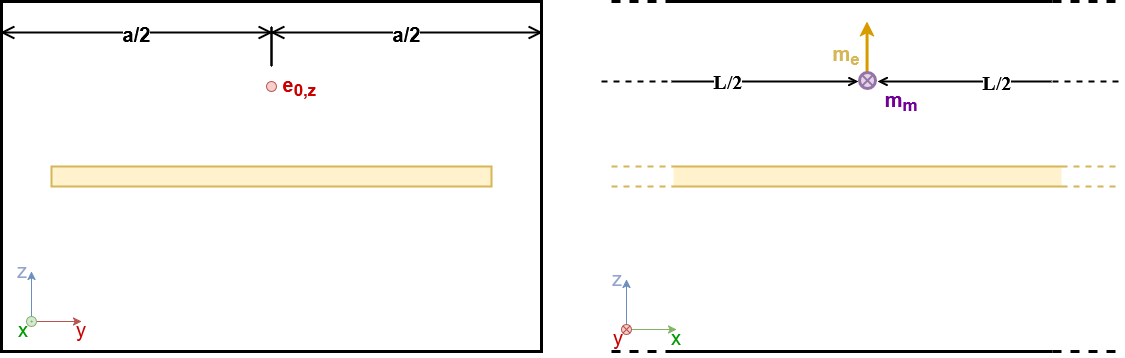
\includegraphics[width=1\linewidth]{Documentation//content//30_simulations//img/sketch_dipoles_tem_cell.png}
    \caption{Dipole moments and measurement point of $e_{0,z}$ in TEM cell}
    \label{fig:sketch_dipoles_tem_cell}
\end{figure}

Using \autoref{eqn:magn_current_curr_loop} the magnetic dipole moment can be expressed as a magnetic current. The resulting $m_{m,mag}$ is shown in \autoref{eqn:m_mymag_ifa}. The phase shift between the magnetic and electric dipole moments $m_{\mathrm{ez}}$ and $m_{\mathrm{my,mag}}$ is always $\frac{\pi}{2}$, which generates the desired TEM wave pattern.

\begin{equation}
    m_{\mathrm{m,mag}}=\mathrm{i}m_{\mathrm{m}}\omega\mu_0
    \label{eqn:m_mymag_ifa}
\end{equation}

The antenna may then be replaced with those two dipole excitations in the center of the upper half of the TEM cell. The magnitude and phase of the fields, as well as the output powers, should remain the same as in the case with the antenna. 

\begin{figure}[h]
    \centering
    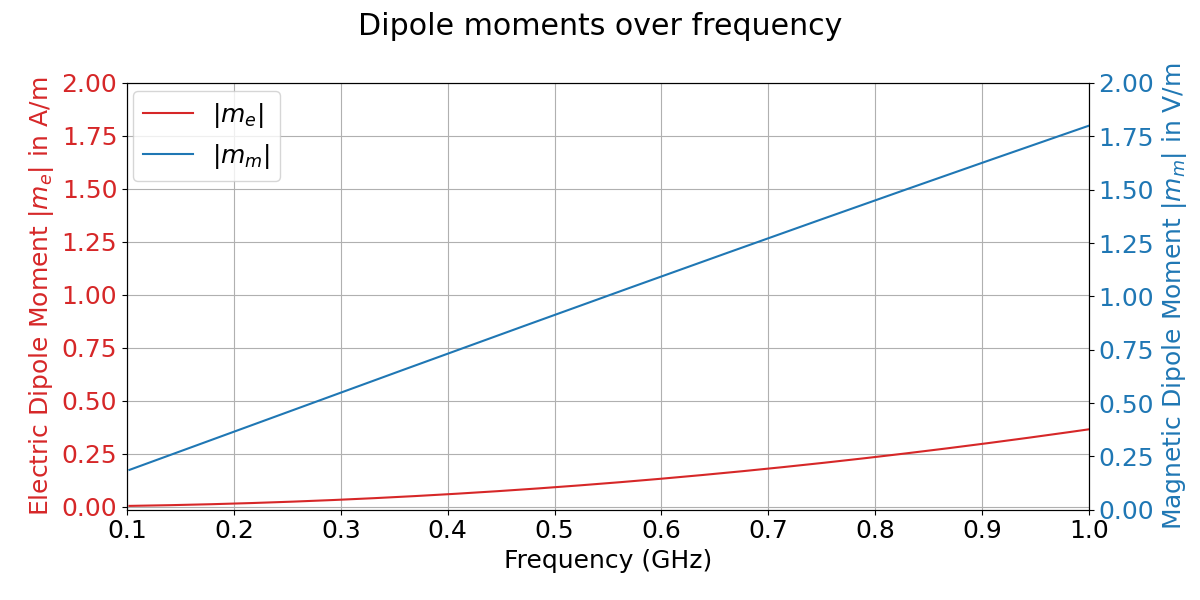
\includegraphics[width=1\linewidth]{Documentation/content/30_simulations/img/dipole_moments_over_freq_ifa.png}
    \caption{Dipole moments over frequency}
    \label{fig:dipole_moments_over_freq_ifa}
\end{figure}

\autoref{fig:dipole_moments_over_freq_ifa} shows the dipole moments over frequency. The electric dipole moment $m_e$ has been normalized to the free-space wave impedance of $377\,\Omega$ to make the dipole moments comparable. The antenna input power has been set to 142588.47\,W, because this leads to an output power of 1\,W at a frequency of 1\,GHz. The magnetic dipole moment is much larger than the electric dipole moment, because the current loop of the antenna is aligned with the TEM cell's magnetic fields, but the line current is not with the TEM electric fields. The magnetic dipole moments rises linearly with the frequency, which is equal to a quadratic increase of power. Only the TEM modes has been considered in the simulation, as other modes disturb the calculations. 

The electric field $\mathbf{e_0}$ is approximated with \autoref{eqn:ifa_e_field_approx} for the purpose of interpolation over frequencies and analytical analysis. \autoref{fig:output_power_e_fields_over_freq_ifa} shows the resulting plot. If any other output power over frequency curves are desired, the formula may easily be modified by considering the quadratic relationship between the electric field and the output power.

\begin{equation}
    a\cdot\mathbf{e_0}=\frac{\sqrt{P_\mathrm{Out}}}{0.0012194}\,\mathrm{\frac{V}{m\sqrt{W}}}
    \label{eqn:ifa_e_field_approx}
\end{equation}

\begin{figure}[h]
    \centering
    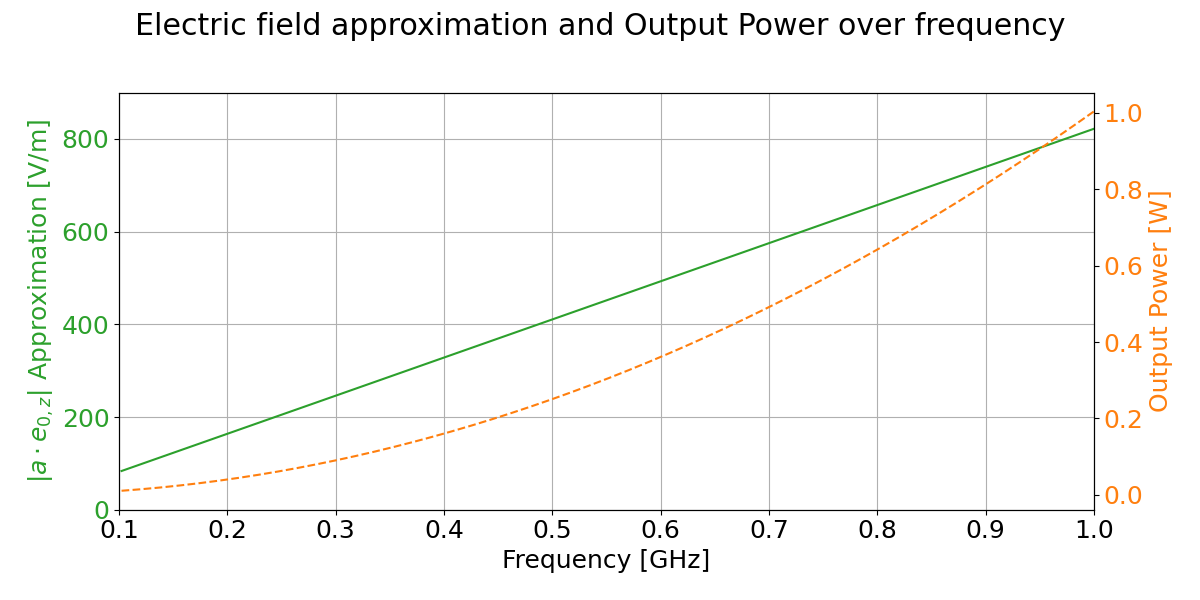
\includegraphics[width=1\linewidth]{Documentation//content//30_simulations//img/output_power_e_fields_over_freq_ifa.png}
    \caption{Output power and electric field over frequency}
    \label{fig:output_power_e_fields_over_freq_ifa}
\end{figure}

\subsection{Center Fed Monopole Antenna}

\begin{figure}[h]
    \centering
    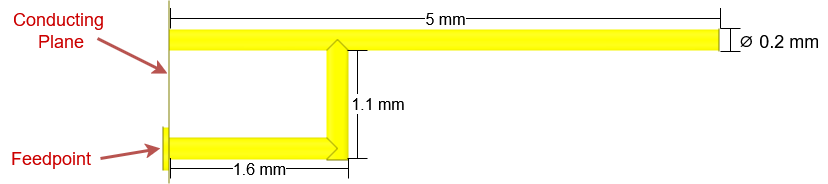
\includegraphics[width=0.75\linewidth]{Documentation//content//30_simulations//img/center_fed_monopole.png}
    \caption{Center fed monopole antenna used in simulation}
    \label{fig:center_fed_monopole}
\end{figure}






\subsection{Offset of source antennas and eddy currents}
